\documentclass[border=0.2cm]{standalone}
\usepackage{tikz}
\begin{document}
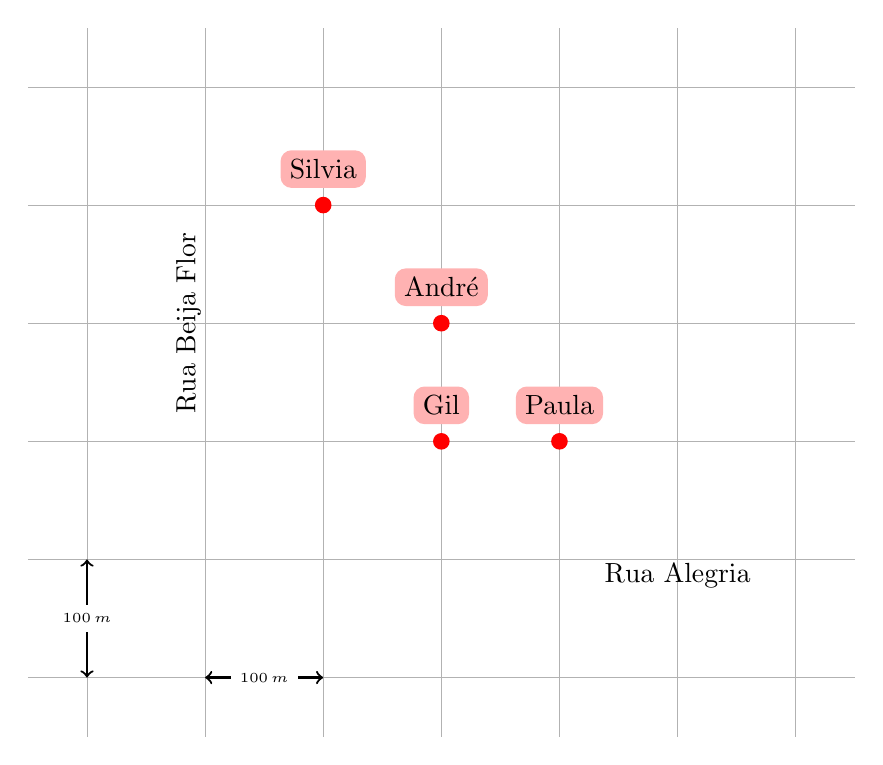
\begin{tikzpicture}[scale=1.5]
\draw[help lines,black!30] (-3.5,-2.5) grid (3.5,3.5);
         
\coordinate (Gil) at (0,0);
\coordinate (André) at (0,1);
\coordinate (Paula) at (1,0);
\coordinate (Silvia) at (-1,2);
\coordinate (R_Beijaflor) at (-2,1);
\coordinate (R_Alegria) at (2,-1);

\foreach \x in {Gil,Paula,André,Silvia} {\fill[red] (\x) circle (2pt) node[above,text=black,fill=red!30,yshift=6pt,rounded corners] {\x};}
\path (R_Beijaflor) node[rotate=90,yshift=6pt] {Rua Beija Flor}; 
\path (R_Alegria) node[yshift=-6pt] {Rua Alegria}; 
\draw[<->,thick] (-3,-1) -- (-3,-2) node[midway,fill=white] {\tiny $100\,m$};
\draw[<->,thick] (-2,-2) -- (-1,-2) node[midway,fill=white] {\tiny $100\,m$};


\end{tikzpicture}

\end{document}